\section{Υλοποιημένα παραδείγματα}
\subparagraph{}
Οι ενότητες που ακολουθούν αφορούν την επίλυση προβλημάτων με διαφορετικές μεθόδους επίλυσης. Τα προβλήματα συγκεντρώθηκαν και επιλύθηκαν με στόχο την σύγκριση των αποτελεσμάτων και την εξαγωγή συμπερασμάτων.Ο πηγαίος των προβλημάτων βρίσκεται στο παρακάτω \en{link} $$\href{https://github.com/gkonto/openmp/}{\en{https://github.com/gkonto/openmp/}}$$
Κάθε πρόβλημα περιέχει υποφακέλους, οπου κάθε υποφάκελος αποτελεί και μια παραλλαγή του προβλήματος.
\begin{center}

\begin{figure}[h]
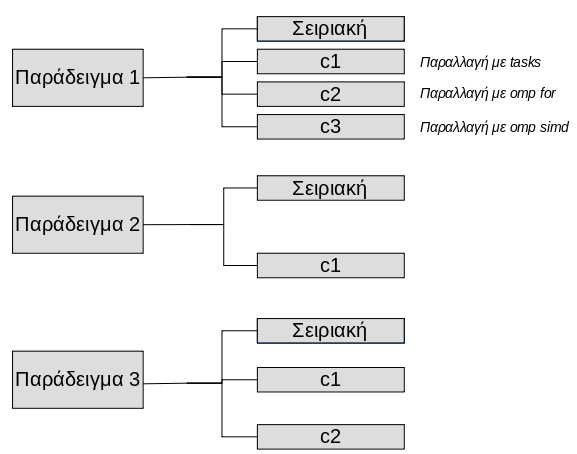
\includegraphics[width=\textwidth]{diarthrosi_example}
\captionsetup{justification=centering, singlelinecheck=false}
\caption{Διάρθρωση παραδειγμάτων στο \en{github}}
\label{fig:diarthrosi_example}
\end{figure}
\end{center}


\subsection{Παράδειγμα διπλασιασμού τιμών στοιχείων πίνακα}
\subparagraph{}
Σε αυτό το παράδειγμα γίνεται ανάλυση του προβλήματος τροποποίησης τιμών ενός διανύσματος. Μελετάται η επίδοση κάθε εναλλακτικής λύσης και σχολιάζονται εργαλεία που αναφέρθηκαν στα προηγούμενα κεφάλαια. Χρησιμοποιείται ένα διάνυσμα μεταβαλλόμενου μεγέθους για κάθε επίλυση, το οποίο αρχικοποιείται στον εξυπηρετητή με τον παρακάτω τρόπο.
\selectlanguage{english}
\begin{lstlisting}[language=C++, caption={\el{Αρχικοποίηση τιμών διανύσματος}} , frame=tlrb]{Name}
void fill_array(int *arr, size_t size) {
    for (size_t k = 0; k < size; ++k) {
            arr[k] = static_cast<int>(k);
    }
}
\end{lstlisting}
\selectlanguage{greek}

Για την επαλήθευση σωστού αποτελέσματος, χρησιμοποιείται η παρακάτω ρουτίνα, που καλείται μετά την εκτέλεση του διπλασιασμού:

\selectlanguage{english}
\begin{lstlisting}[language=C++, caption={\el{Αρχικοποίηση τιμών διανύσματος}} , frame=tlrb]{Name}
void verify(int *arr, size_t size) {
	for (size_t k = 0; k < size; ++k) {
		if (arr[k] != k * 2) {
        	printf('Error in position %ld.
        		Got %d, 
        		expected %ld\n', 
        		k, 
        		arr[k], 
        		k * 2);
			exit(1);
		}
	}
}
\end{lstlisting}
\selectlanguage{greek}

Η μεταγλώττιση του κώδικα έγινε με μεταγλωττιστή \emph{\en{g++-7}} και τις επιλογές:$-Wall -o exec -O0$. Οι παραλλαγές εκτέλεσης του προβλήματος χωρίζονται σε δύο κατηγορίες, σε αυτές που απαιτείται αντιγραφή δεδομένων από τον εξυπηρετητή στον επιταχυντή, και από αυτές που δεσμεύουν μνήμη απευθείας στον επιταχυντή.

\subsubsection{Σειριακή εκτέλεση}
\subparagraph{}
Για το σειριακό υπολογισμό, η ρουτίνα που εκτελέστηκε ήταν η εξής:

\selectlanguage{english}
\begin{lstlisting}[language=C++, caption={\el{Αρχικοποίηση τιμών διανύσματος}} , frame=tlrb]{Name}
void double_elements(int *A, size_t size) {
    for (size_t i = 0; i < size; ++i) {
            A[i] = A[i] * 2;
    }
}
\end{lstlisting}
\selectlanguage{greek}
Οι χρόνοι εκτέλεσης που καταγράφηκαν εμφανίζονται στον παρακάτων πίνακα:

\begin{center}
\begin{table}[htbp]
\captionsetup{justification=raggedright,
singlelinecheck=false
}
\caption{ Καταγραφή χρόνων εκτέλεσης παραδειγμάτων}
\def\arraystretch{1.5}
\begin{tabular}{| p{0.25\textwidth} | p{0.25\textwidth}|}
 \textbf{Αριθμός στοιχείων πίνακα\cellcolor[HTML]{D0D0D0}} & \textbf{Χρόνος εκτέλεσης (\emph{\en{sec}}) }\cellcolor[HTML]{D0D0D0} \\
\hline
 100000 & 0.002  \\
\hline
1000000 & 0.0097 \\
\hline
10000000 & 0.098  \\
\hline
100000000 &  0.980\\
\hline
200000000 & 1.978 \\
\hline
300000000 & 2.968 \\
\hline
\end{tabular}
\end{table}
\end{center}


\subsubsection{Υλοποιήσεις που απαιτούν αντιγραφή μνήμης}
\subparagraph{}
Τα παραδείγματα που ακολουθούν αφορούν υλοποίηση του προβλήματος με μεθόδους που απαιτούν αντιγραφή δεδομένων ανάμεσα στον εξυπηρετητή και στον επιταχυντή. Για την αντιγραφή των δεδομένων χρησιμοποιούνται οι φράσεις που υποστηρίζονται από την οδηγία \emph{\en{map}} και αναφέρθηκαν στα προηγούμενα κεφάλαια.

\paragraph{Παράλληλη εκτέλεση 1}
\subparagraph{}
Για τον υπολογισμό, η ρουτίνα που εκτελέστηκε ήταν η εξής:

\selectlanguage{english}
\begin{lstlisting}[language=C++, caption={\el{Αρχικοποίηση τιμών διανύσματος}} , frame=tlrb]{Name}
void double_elements(int *A, size_t size) {
#pragma omp target map(A[:size] )
    for (size_t i = 0; i < size; ++i) {
            A[i] = A[i] * 2;
    }
}
\end{lstlisting}
\selectlanguage{greek}
\begin{center}
\begin{table}[htbp]
\captionsetup{justification=raggedright,
singlelinecheck=false
}
\caption{ Καταγραφή χρόνων εκτέλεσης παραδειγμάτων}
\def\arraystretch{1.5}
\begin{tabular}{| p{0.25\textwidth} | p{0.25\textwidth}|}
 \textbf{Αριθμός στοιχείων πίνακα\cellcolor[HTML]{D0D0D0}} & \textbf{Χρόνος εκτέλεσης (\emph{\en{sec}}) }\cellcolor[HTML]{D0D0D0} \\
\hline
100000 & 0.971  \\
\hline
1000000 & 1.838 \\
\hline
10000000 & 10.177 \\
\hline
\end{tabular}
\end{table}
\end{center}

\paragraph{Παράλληλη εκτέλεση 2}
\subparagraph{}
Για τον υπολογισμό, η ρουτίνα που εκτελέστηκε ήταν η εξής:

\selectlanguage{english}
\begin{lstlisting}[language=C++, caption={\el{Αρχικοποίηση τιμών διανύσματος}} , frame=tlrb]{Name}
void double_elements(int *A, size_t size) {
#pragma omp target map(A[:size], flag)
	{
		#pragma omp parallel for
		for (size_t i = 0; i < size; ++i) {
        	A[i] = A[i] * 2;
	    }
    }
}
\end{lstlisting}
\selectlanguage{greek}
\begin{center}
\begin{table}[htbp]
\captionsetup{justification=raggedright,
singlelinecheck=false
}
\caption{ Καταγραφή χρόνων εκτέλεσης παραδειγμάτων}
\def\arraystretch{1.5}
\begin{tabular}{| p{0.25\textwidth} | p{0.25\textwidth}|}
 \textbf{Αριθμός στοιχείων πίνακα\cellcolor[HTML]{D0D0D0}} & \textbf{Χρόνος εκτέλεσης (\emph{\en{sec}}) }\cellcolor[HTML]{D0D0D0} \\
\hline
100000 & 0.885 \\
\hline
1000000 & 0.971 \\
\hline
10000000 & 2.153 \\
\hline
100000000 & 13.566 \\
\hline
\end{tabular}
\end{table}
\end{center}


\paragraph{Παράλληλη εκτέλεση 2}
\subparagraph{}
Για τον υπολογισμό, η ρουτίνα που εκτελέστηκε ήταν η εξής:

\selectlanguage{english}
\begin{lstlisting}[language=C++, caption={\el{Αρχικοποίηση τιμών διανύσματος}} , frame=tlrb]{Name}
void double_elements(int *A, size_t size) {
#pragma omp target parallel map(A[:size], flag)
	{
		for (size_t i = 0; i < size; ++i) {
        	A[i] = A[i] * 2;
	    }
    }
}
\end{lstlisting}
\selectlanguage{greek}
\begin{center}
\begin{table}[htbp]
\captionsetup{justification=raggedright,
singlelinecheck=false
}
\caption{ Καταγραφή χρόνων εκτέλεσης παραδειγμάτων}
\def\arraystretch{1.5}
\begin{tabular}{| p{0.25\textwidth} | p{0.25\textwidth}|}
 \textbf{Αριθμός στοιχείων πίνακα\cellcolor[HTML]{D0D0D0}} & \textbf{Χρόνος εκτέλεσης (\emph{\en{sec}}) }\cellcolor[HTML]{D0D0D0} \\
\hline
100000 & 0.885 \\
\hline
1000000 & 0.971 \\
\hline
10000000 & 2.153 \\
\hline
100000000 & 13.566 \\
\hline
\end{tabular}
\end{table}
\end{center}


\paragraph{Παράλληλη εκτέλεση 2}
\subparagraph{}
Για τον υπολογισμό, η ρουτίνα που εκτελέστηκε ήταν η εξής:

\selectlanguage{english}
\begin{lstlisting}[language=C++, caption={\el{Αρχικοποίηση τιμών διανύσματος}} , frame=tlrb]{Name}
void double_elements(int *A, size_t size) {
#pragma omp target parallel for simd map(A[:size], flag)
	{
		for (size_t i = 0; i < size; ++i) {
        	A[i] = A[i] * 2;
	    }
    }
}
\end{lstlisting}
\selectlanguage{greek}
\begin{center}
\begin{table}[htbp]
\captionsetup{justification=raggedright,
singlelinecheck=false
}
\caption{ Καταγραφή χρόνων εκτέλεσης παραδειγμάτων}
\def\arraystretch{1.5}
\begin{tabular}{| p{0.25\textwidth} | p{0.25\textwidth}|}
 \textbf{Αριθμός στοιχείων πίνακα\cellcolor[HTML]{D0D0D0}} & \textbf{Χρόνος εκτέλεσης (\emph{\en{sec}}) }\cellcolor[HTML]{D0D0D0} \\
\hline
100000 & 0.885 \\
\hline
1000000 & 0.971 \\
\hline
10000000 & 2.153 \\
\hline
100000000 & 13.566 \\
\hline
\end{tabular}
\end{table}
\end{center}



\paragraph{Παράλληλη εκτέλεση 2}
\subparagraph{}
Για τον υπολογισμό, η ρουτίνα που εκτελέστηκε ήταν η εξής:

\selectlanguage{english}
\begin{lstlisting}[language=C++, caption={\el{Αρχικοποίηση τιμών διανύσματος}} , frame=tlrb]{Name}
void double_elements(int *A, size_t size) {
#pragma omp target parallel simd map(A[:size], flag)
	{
		for (size_t i = 0; i < size; ++i) {
        	A[i] = A[i] * 2;
	    }
    }
}
\end{lstlisting}
\selectlanguage{greek}
\begin{center}
\begin{table}[htbp]
\captionsetup{justification=raggedright,
singlelinecheck=false
}
\caption{ Καταγραφή χρόνων εκτέλεσης παραδειγμάτων}
\def\arraystretch{1.5}
\begin{tabular}{| p{0.25\textwidth} | p{0.25\textwidth}|}
 \textbf{Αριθμός στοιχείων πίνακα\cellcolor[HTML]{D0D0D0}} & \textbf{Χρόνος εκτέλεσης (\emph{\en{sec}}) }\cellcolor[HTML]{D0D0D0} \\
\hline
100000 & 0.885 \\
\hline
1000000 & 0.971 \\
\hline
10000000 & 2.153 \\
\hline
100000000 & 13.566 \\
\hline
\end{tabular}
\end{table}
\end{center}

\paragraph{Παράλληλη εκτέλεση 2}
\subparagraph{}
Για τον υπολογισμό, η ρουτίνα που εκτελέστηκε ήταν η εξής:

\selectlanguage{english}
\begin{lstlisting}[language=C++, caption={\el{Αρχικοποίηση τιμών διανύσματος}} , frame=tlrb]{Name}
void double_elements(int *A, size_t size) {
#pragma omp target teams distribute map(A[:size], flag)
	{
		for (size_t i = 0; i < size; ++i) {
        	A[i] = A[i] * 2;
	    }
    }
}
\end{lstlisting}
\selectlanguage{greek}
\begin{center}
\begin{table}[htbp]
\captionsetup{justification=raggedright,
singlelinecheck=false
}
\caption{ Καταγραφή χρόνων εκτέλεσης παραδειγμάτων}
\def\arraystretch{1.5}
\begin{tabular}{| p{0.25\textwidth} | p{0.25\textwidth}|}
 \textbf{Αριθμός στοιχείων πίνακα\cellcolor[HTML]{D0D0D0}} & \textbf{Χρόνος εκτέλεσης (\emph{\en{sec}}) }\cellcolor[HTML]{D0D0D0} \\
\hline
100000 & 0.885 \\
\hline
1000000 & 0.971 \\
\hline
10000000 & 2.153 \\
\hline
100000000 & 13.566 \\
\hline
\end{tabular}
\end{table}
\end{center}

\paragraph{Παράλληλη εκτέλεση 2}
\subparagraph{}
Για τον υπολογισμό, η ρουτίνα που εκτελέστηκε ήταν η εξής:

\selectlanguage{english}
\begin{lstlisting}[language=C++, caption={\el{Αρχικοποίηση τιμών διανύσματος}} , frame=tlrb]{Name}
void double_elements(int *A, size_t size) {
#pragma omp target teams distribute parallel for map(A[:size], flag)
	{
		for (size_t i = 0; i < size; ++i) {
        	A[i] = A[i] * 2;
	    }
    }
}
\end{lstlisting}
\selectlanguage{greek}
\begin{center}
\begin{table}[htbp]
\captionsetup{justification=raggedright,
singlelinecheck=false
}
\caption{ Καταγραφή χρόνων εκτέλεσης παραδειγμάτων}
\def\arraystretch{1.5}
\begin{tabular}{| p{0.25\textwidth} | p{0.25\textwidth}|}
 \textbf{Αριθμός στοιχείων πίνακα\cellcolor[HTML]{D0D0D0}} & \textbf{Χρόνος εκτέλεσης (\emph{\en{sec}}) }\cellcolor[HTML]{D0D0D0} \\
\hline
100000 & 0.885 \\
\hline
1000000 & 0.971 \\
\hline
10000000 & 2.153 \\
\hline
100000000 & 13.566 \\
\hline
\end{tabular}
\end{table}
\end{center}


\paragraph{Παράλληλη εκτέλεση 2}
\subparagraph{}
Για τον υπολογισμό, η ρουτίνα που εκτελέστηκε ήταν η εξής:

\selectlanguage{english}
\begin{lstlisting}[language=C++, caption={\el{Αρχικοποίηση τιμών διανύσματος}} , frame=tlrb]{Name}
void double_elements(int *A, size_t size) {
#pragma omp target teams distribute simd map(A[:size], flag)
	{
		for (size_t i = 0; i < size; ++i) {
        	A[i] = A[i] * 2;
	    }
    }
}
\end{lstlisting}
\selectlanguage{greek}
\begin{center}
\begin{table}[htbp]
\captionsetup{justification=raggedright,
singlelinecheck=false
}
\caption{ Καταγραφή χρόνων εκτέλεσης παραδειγμάτων}
\def\arraystretch{1.5}
\begin{tabular}{| p{0.25\textwidth} | p{0.25\textwidth}|}
 \textbf{Αριθμός στοιχείων πίνακα\cellcolor[HTML]{D0D0D0}} & \textbf{Χρόνος εκτέλεσης (\emph{\en{sec}}) }\cellcolor[HTML]{D0D0D0} \\
\hline
100000 &  \\
\hline
1000000 &  \\
\hline
10000000 &  \\
\hline
100000000 &  \\
\hline
\end{tabular}
\end{table}
\end{center}


\paragraph{Παράλληλη εκτέλεση 2}
\subparagraph{}
Για τον υπολογισμό, η ρουτίνα που εκτελέστηκε ήταν η εξής:

\selectlanguage{english}
\begin{lstlisting}[language=C++, caption={\el{Αρχικοποίηση τιμών διανύσματος}} , frame=tlrb]{Name}
void double_elements(int *A, size_t size) {
#pragma omp target teams distribute parallel for simd map(A[:size], flag)
	{
		for (size_t i = 0; i < size; ++i) {
        	A[i] = A[i] * 2;
	    }
    }
}
\end{lstlisting}
\selectlanguage{greek}
\begin{center}
\begin{table}[htbp]
\captionsetup{justification=raggedright,
singlelinecheck=false
}
\caption{ Καταγραφή χρόνων εκτέλεσης παραδειγμάτων}
\def\arraystretch{1.5}
\begin{tabular}{| p{0.25\textwidth} | p{0.25\textwidth}|}
 \textbf{Αριθμός στοιχείων πίνακα\cellcolor[HTML]{D0D0D0}} & \textbf{Χρόνος εκτέλεσης (\emph{\en{sec}}) }\cellcolor[HTML]{D0D0D0} \\
\hline
100000 & 0.885 \\
\hline
1000000 & 0.971 \\
\hline
10000000 & 2.153 \\
\hline
100000000 & 13.566 \\
\hline
\end{tabular}
\end{table}
\end{center}



\subsubsection{Υλοποιήσεις που δεσμεύουν μνήμη απευθείας στον επιταχυντή}
\subparagraph{}
Στις υλοποιήσεις αυτής της ενότητας δεν απαιτείται αντιγραφή δεδομένων μνήμης ανάμεσα στα περιβάλλοντα δεδομένων του επιταχυντή και του εξυπηρετητή, καθώς η μνήμη δεσμεύεται απευθείας στον επιταχυντή μέσω της οδηγίας \emph{\en{omp\_target\_alloc}}. Σε αυτή την εκτέλεση, δεσμεύεται μνήμη για το διάνυσμα απευθείας στη συσκευή στόχου. Με αυτό τον τρόπο αποφεύγονται εργασίες αντιγραφής ανάμεσα στα δύο μέσα.
\clearpage
\selectlanguage{english}
\begin{lstlisting}[language=C++, caption={\el{Κώδικας αρχικοποίησης διανύσματος στη συσκευή στόχου και επαλήθευση ομαλής εκτέλεσης}} , frame=tlrb]{Name}
    std::cout << "Device: " << device << std::endl;
    int *a = (int *)omp_target_alloc(sizeof(int) * o.size, device);
    if (!a) {
            std::cout << "Could not allocate memory for array"
             << std::endl;
            exit(1);
    } else {
            std::cout << "Successful allocation" << std::endl;
    }
#pragma omp target is_device_ptr(a)
    for (size_t i = 0; i < o.size; ++i) {
            a[i] = static_cast<int>(i);
    }
    //Count time
    auto start = omp_get_wtime();
    double_elements(a, o.size);
    auto end = omp_get_wtime();
    std::cout << "Starting verification" << std::endl;
#pragma omp target is_device_ptr(a)
    for (size_t i = 0; i < o.size; ++i) {
            if (a[i] != i * 2) {
                    exit(1);
            }
    }
    std::cout << "Successful verification" << std::endl;
    omp_target_free(a, device);
\end{lstlisting}
\selectlanguage{greek}

\clearpage
\paragraph{Παραλλαγή 1}
\subparagraph{}
Για τον υπολογισμό, η ρουτίνα που εκτελέστηκε ήταν η εξής:

\selectlanguage{english}
\begin{lstlisting}[language=C++, caption={\el{Εκτέλεση υπολογισμών}} , frame=tlrb]{Name}
void double_elements(int *A, size_t size) {
#pragma omp target is_device_ptr(A)
        {
        #pragma omp parallel for
                for (size_t i = 0; i < size; ++i) {
                        A[i] = A[i] * 2;
                }
        }
}
\end{lstlisting}
\selectlanguage{greek}

\begin{center}
\begin{table}[htbp]
\captionsetup{justification=raggedright,
singlelinecheck=false
}
\caption{ Καταγραφή χρόνων εκτέλεσης παραδειγμάτων}
\def\arraystretch{1.5}
\begin{tabular}{| p{0.25\textwidth} | p{0.25\textwidth}|}
 \textbf{Αριθμός στοιχείων πίνακα\cellcolor[HTML]{D0D0D0}} & \textbf{Χρόνος εκτέλεσης (\emph{\en{sec}}) }\cellcolor[HTML]{D0D0D0} \\
\hline
100000 & 0.016400 \\
\hline
1000000 & 0.118455 \\
\hline
10000000 & 1.179038 \\
\hline
100000000 & 11.780315 \\
\hline
\end{tabular}
\end{table}
\end{center}




\paragraph{Παραλλαγή}
\subparagraph{}
Για τον υπολογισμό, η ρουτίνα που εκτελέστηκε ήταν η εξής:

\selectlanguage{english}
\begin{lstlisting}[language=C++, caption={\el{Εκτέλεση υπολογισμών}} , frame=tlrb]{Name}
void double_elements(int *A, size_t size) {
#pragma omp target parallel for is_device_ptr(A)
        for (size_t i = 0; i < size; ++i) {
                A[i] = A[i] * 2;
        }
}

\end{lstlisting}
\selectlanguage{greek}

\begin{center}
\begin{table}[htbp]
\captionsetup{justification=raggedright,
singlelinecheck=false
}
\caption{ Καταγραφή χρόνων εκτέλεσης παραδειγμάτων}
\def\arraystretch{1.5}
\begin{tabular}{| p{0.25\textwidth} | p{0.25\textwidth}|}
 \textbf{Αριθμός στοιχείων πίνακα\cellcolor[HTML]{D0D0D0}} & \textbf{Χρόνος εκτέλεσης (\emph{\en{sec}}) }\cellcolor[HTML]{D0D0D0} \\
\hline

\end{tabular}
\end{table}
\end{center}




\paragraph{Παραλλαγή 2}
\subparagraph{}
Για τον υπολογισμό, η ρουτίνα που εκτελέστηκε ήταν η εξής:

\selectlanguage{english}
\begin{lstlisting}[language=C++, caption={\el{Εκτέλεση υπολογισμών}} , frame=tlrb]{Name}
void double_elements(int *A, size_t size) {
#pragma omp target teams distribute is_device_ptr(A)
        for (size_t i = 0; i < size; ++i) {
                A[i] = A[i] * 2;
        }
}

\end{lstlisting}
\selectlanguage{greek}

\begin{center}
\begin{table}[htbp]
\captionsetup{justification=raggedright,
singlelinecheck=false
}
\caption{ Καταγραφή χρόνων εκτέλεσης παραδειγμάτων}
\def\arraystretch{1.5}
\begin{tabular}{| p{0.25\textwidth} | p{0.25\textwidth}|}
 \textbf{Αριθμός στοιχείων πίνακα\cellcolor[HTML]{D0D0D0}} & \textbf{Χρόνος εκτέλεσης (\emph{\en{sec}}) }\cellcolor[HTML]{D0D0D0} \\
\hline
100000 &  \\
\hline
1000000 &  \\
\hline
10000000 &  \\
\hline
100000000 &  \\
\hline
200000000 &  \\
\hline
\end{tabular}
\end{table}
\end{center}

\clearpage
\paragraph{Παραλλαγή 3}
\subparagraph{}
Για τον υπολογισμό, η ρουτίνα που εκτελέστηκε ήταν η εξής:

\selectlanguage{english}
\begin{lstlisting}[language=C++, caption={\el{Εκτέλεση υπολογισμών}} , frame=tlrb]{Name}
void double_elements(int *A, size_t size) {
#pragma omp target teams distribute parallel for is_device_ptr(A)
        for (size_t i = 0; i < size; ++i) {
                A[i] = A[i] * 2;
        }
}
\end{lstlisting}
\selectlanguage{greek}

\begin{center}
\begin{table}[htbp]
\captionsetup{justification=raggedright,
singlelinecheck=false
}
\caption{ Καταγραφή χρόνων εκτέλεσης παραδειγμάτων}
\def\arraystretch{1.5}
\begin{tabular}{| p{0.25\textwidth} | p{0.25\textwidth}|}
 \textbf{Αριθμός στοιχείων πίνακα\cellcolor[HTML]{D0D0D0}} & \textbf{Χρόνος εκτέλεσης (\emph{\en{sec}}) }\cellcolor[HTML]{D0D0D0} \\
\hline
100000 &  \\
\hline
1000000 &  \\
\hline
10000000 &  \\
\hline
100000000 &  \\
\hline
200000000 &  \\
\hline
300000000 &  \\
\hline
\end{tabular}
\end{table}
\end{center}

\paragraph{Παραλλαγή 4}
\subparagraph{}
Για τον υπολογισμό, η ρουτίνα που εκτελέστηκε ήταν η εξής:

\selectlanguage{english}
\begin{lstlisting}[language=C++, caption={\el{Εκτέλεση υπολογισμών}} , frame=tlrb]{Name}
void double_elements(int *A, size_t size) {
#pragma omp target teams distribute simd is_device_ptr(A)
        for (size_t i = 0; i < size; ++i) {
                A[i] = A[i] * 2;
        }
}
\end{lstlisting}
\selectlanguage{greek}


\begin{center}
\begin{table}[htbp]
\captionsetup{justification=raggedright,
singlelinecheck=false
}
\caption{ Καταγραφή χρόνων εκτέλεσης παραδειγμάτων}
\def\arraystretch{1.5}
\begin{tabular}{| p{0.25\textwidth} | p{0.25\textwidth}|}
 \textbf{Αριθμός στοιχείων πίνακα\cellcolor[HTML]{D0D0D0}} & \textbf{Χρόνος εκτέλεσης (\emph{\en{sec}}) }\cellcolor[HTML]{D0D0D0} \\
\hline
100000 &  \\
\hline
1000000 &  \\
\hline
10000000 &  \\
\hline
100000000 &  \\
\hline
200000000 &  \\
\hline
300000000 &  \\
\hline
\end{tabular}
\end{table}
\end{center}



\paragraph{Παραλλαγή 4}
\subparagraph{}
Για τον υπολογισμό, η ρουτίνα που εκτελέστηκε ήταν η εξής:

\selectlanguage{english}
\begin{lstlisting}[language=C++, caption={\el{Εκτέλεση υπολογισμών}} , frame=tlrb]{Name}
void double_elements(int *A, size_t size) {
#pragma omp target teams distribute parallel for simd is_device_ptr(A)
        for (size_t i = 0; i < size; ++i) {
                A[i] = A[i] * 2;
        }
}
\end{lstlisting}
\selectlanguage{greek}


\begin{center}
\begin{table}[htbp]
\captionsetup{justification=raggedright,
singlelinecheck=false
}
\caption{ Καταγραφή χρόνων εκτέλεσης παραδειγμάτων}
\def\arraystretch{1.5}
\begin{tabular}{| p{0.25\textwidth} | p{0.25\textwidth}|}
 \textbf{Αριθμός στοιχείων πίνακα\cellcolor[HTML]{D0D0D0}} & \textbf{Χρόνος εκτέλεσης (\emph{\en{sec}}) }\cellcolor[HTML]{D0D0D0} \\
\hline
100000 &  \\
\hline
1000000 &  \\
\hline
10000000 &  \\
\hline
100000000 &  \\
\hline
200000000 &  \\
\hline
300000000 &  \\
\hline
\end{tabular}
\end{table}
\end{center}

\subsubsection{Αποτελέσματα και σχόλια}
\subparagraph{}
\begin{tikzpicture}
\begin{axis}[
    title={Τίτλος},
    xlabel={Αριθμός στοιχείων διανύσματος},
    legend cell align = {left},
    ylabel={Χρόνος εκτέλεσης \emph{\en{sec}}},
    xmin=100000, xmax=300000000,
    ymin=0, ymax=5,
    xtick={100000,100000000, 200000000, 300000000},
    ytick={0,1,2,3,4,5},
    legend pos= outer north east,
    ymajorgrids=true,
    width = 0.65\textwidth,
    grid style=dashed,
]

\addplot[
    color=blue,
    mark=triangle,
    ]
    coordinates {
    (100000,0.00244)(1000000, 0.009742)(10000000, 0.098103)(100000000, 0.98088)(100000000, 0.981602)(200000000, 1.978147) (300000000, 2.968849)
    };
    \addlegendentry{Σειριακή}
    
    \addplot[
    color=red,
    mark=square,
    ]
    coordinates {
    (100000,0.971228)(1000000, 1.838727)(10000000,10.177887)
    };
    \addlegendentry{Εκτέλεση 4.1.2.1}
        
    \addplot[
    color=green,
    mark=square,
    ]
    coordinates {
    (100000,0.885608)(1000000, 0.971478)(10000000, 2.153557)(100000000, 13.566249)
    };
    \addlegendentry{Εκτέλεση 4.1.2.2}
    
        \addplot[
    color=black,
    mark=*,
    ]
    coordinates {
    (100000,0.016400)(1000000, 0.118455)(10000000, 1.179038)(100000000, 11.780315)
    };
    \addlegendentry{Εκτέλεση 4.1.3.1}
    
\addplot[
    color=black,
    mark=x,
    ]
    coordinates {
    (100000,0.006752)(1000000, 0.029761)(10000000, 0.202267)(100000000, 1.984212)(200000000, 3.934013)
    };
    \addlegendentry{Εκτέλεση 4.1.3.2}
    
    \addplot[
    color=purple,
    mark=square,
    ]
    coordinates {
    (100000,0.004939)(1000000, 0.008046)(10000000,0.032330 )(100000000,0.299236 )(200000000, 0.631952)(300000000,0.954900)
    };
    \addlegendentry{Εκτέλεση 4.1.3.3}
    
        \addplot[
    color=cyan,
    mark=square,
    ]
    coordinates {
    (100000,0.006792)(1000000, 0.029622)(10000000,0.201454 )(100000000, 1.977574)(200000000, 3.920045)(300000000,5.908174)
    };
    \addlegendentry{Εκτέλεση 4.1.3.4}
\end{axis}
\end{tikzpicture}


\subsection{Υπολογισμός εσωτερικού γινόμενου}
\subparagraph{}

Δες \emph{\en{pdf}} σελ 304

\subsection{Πρόβλημα προσπέλασης συνδεδεμένης λίστας}
\subparagraph{}
Το παρακάτω παράδειγμα διατρέχει μια συνδεδεμένη λίστα, όπου κάθε κόμβος της θα χρησιμοποιεί τα δεδομένα του για την εκτέλεση μια μεμονομένης διεργασίας, ξεχωριστής από τους υπόλοιπους κόμβους. Στην προκειμένη περίπτωση τα δεδομένα των κόμβων είναι ένας ακέραιος αριθμός.


Κάθε κόμβος της λίστας αρχικοποιείται με τον αριθμό \textbf{33}. Η κάθε εργασία θα έχει ως στόχο τον υπολογισμό του αριθμού της ακολουθίας \emph{\en{fibonacci}}.
Το μέγεθος του προβλήματος επηρεάζεται από τον αριθμό των συνολικών κόμβων της λίστας και όχι απο την τιμή που πρέπει να υπολογιστεί για την ακολουθία \emph{fibonacci}η οποία είναι πάντα σταθερή και ίση με \textbf{33}.
Η ανεξαρτησία των κόμβων διευκολύνει τον παράλληλο υπολογισμό. Ωστόσο, οι συνδεδεμένες λίστες διετρέχονται σειριακά, καταστώντας τον παραλληλισμό μή εφικτό.
\ \\
\begin{center}

\selectlanguage{english}
\begin{lstlisting}[ tabsize = 2, basicstyle=\small, language=C++, caption={\el{Συνάρτηση αρχικοποίησης κόμβων}}, frame = tb]{Name}
		
Node *init_nodes(int num, int value) {
     Node *head = new Node(value);
     Node *temp = nullptr;
 
     Node *p = head;
     for (int i = 0; i < num; ++i) {
         temp =  new Node(value);
         p->next_ = temp;
         p = temp;
         p->data_ = value;
     }
     p->next_ = nullptr;
     return head;
 }
\end{lstlisting}
\end{center}
\clearpage
\selectlanguage{english}
\begin{lstlisting}[ tabsize = 2, basicstyle=\small, language=C++, caption={\el{Δομή κόμβου συνδεδεμένης λίστας}}, frame = tb]{Name}
 struct Node {
     Node *next_ = nullptr; // pointer to the next node
     int data_ = 0;         // the stored data is an integer in this example
 };
\end{lstlisting}
\selectlanguage{greek}

Λύση στο πρόβλημα, αποτελεί η αρχική προσπέλαση της λίστας με σκοπό την εισαγωγή των κόμβων της σε διάνυσμα και στη συνέχεια η παραλληλη εκτέλεση μέσω οδηγίας διαμοιρασμού εργασίας βρόγχου - \emph{\en{for}}.
Αυτή η λύση ωστόσο προκαλεί τα παρακάτω προβλήματα:
\begin{enumerate}
\item Γίνεται αρχικά μία προσπέλαση σε όλους τους κόμβους της λιστας, με σκοπό την αποθήκευση τους σε ένα σειριακό μέσο αποθήκευσης.
\item Σε περίπτωση που ο αριθμός των κόμβων της λίστας δεν ειναι γνωστός, θα πρέπει να γίνουν περισσότερες απο μία δεσμεύσεις μνήμης \emph{\en{malloc}}, διαδικασίας χρονοβόρας.
\item Γίνεται άσκοπη δέσμευση μνήμης για το διάνυσμα που θα αποθηκευτούν οι κόμβοι. Σε περίπτωση μεγάλου αριθμού κόμβων λίστας, αυτό μπορει να αποτελέσει πρόβλημα.

\end{enumerate}
\clearpage
\selectlanguage{english}
\begin{lstlisting}[ tabsize = 2, basicstyle=\small, language=C++, caption={\el{Λύση προβλήματος συνδεδεμένης λίστας με χρηση οδηγίας διαμοιρασμού εργασίας} }, frame = tb]{Name}
	 std::vector<Node *> nodes_(o.num_nodes_);  
     for (int i = 0; i < o.num_nodes_; ++i) {
         nodes_[i] = p;
         p = p->next_;
     }
	 #pragma omp parallel
     {
 		#pragma omp for schedule(static, 1) 
         for (int i = 0; i < o.num_nodes_; ++i) {
             fib(p->data_);
         }
     }
\end{lstlisting}
\selectlanguage{greek}

Τα παραπάνω προβλήματα επιλύονται με την χρήση διεργασιών. Ο κώδικας διέρχεται μια φορά από την λίστα με σκοπό την δημουργία μιας διεργασίας για κάθε κόμβο. Οι διεργασίας ξεκινούν να εκτελούνται αυτόματα, μόλις βρεθεί μή ενεργό νήμα, δηλαδή μόλις ένα νήμα φτάσει στο φράγμα κώδικα.

\ \\
\selectlanguage{english}
\begin{lstlisting}[ tabsize = 4, basicstyle=\small, language=C++, caption={\el{Λύση προβλήματος συνδεδεμένης λίστας με χρηση οδηγίας διαμοιρασμού εργασίας} }, frame = tb]{Name}
   #pragma omp parallel
   {
   	#pragma omp single
   	{
   		Node *p = head;
   		while (p) {
   			#pragma omp task firstprivate(p)
   				fib(p->data_);
   			p = p->next_;
   		}
   	}
   }

\end{lstlisting}

\clearpage
\selectlanguage{greek}

\subsubsection{ Αποτελέσματα εκτέλεσης}
\subparagraph{}
Στα παρακάτω διαγράμματα γίνεται σύγκριση με αποτελέσματα απο του αλγόριθμου με διαφορετικές μεθόδους.

\begin{tikzpicture}
\begin{axis}[
    title={Τίτλος},
    xlabel={Αριθμός κόμβων},
    legend cell align = {left},
    ylabel={Χρόνος εκτέλεσης \emph{\en{sec}}},
    xmin=30, xmax=90,
    ymin=0, ymax=7,
    xtick={0, 30, 40, 50, 60, 70, 80, 90},
    ytick={0,1,2,3,4,5,6, 7},
    legend pos= outer north east,
    ymajorgrids=true,
    width = 0.65\textwidth,
    grid style=dashed,
]

\addplot[
    color=blue,
    mark=triangle,
    ]
    coordinates {
    (30,1.92)(40,2.55)(50,3.16)(60,3.8)(70,4.41)(80,5.03)(90,6.65)
    };
    \addlegendentry{Σειριακή}


    \addplot[
    color=red,
    mark=*,
    ]
    coordinates {
    (30,1.92)(40,2.46)(50,3.06)(60,3.73)(70,4.59)(80,4.91)(90,5.51)
    };
	\addlegendentry{\en{c1 - Threads} 1}

        \addplot[
    color=green,
    mark=square,
    ]
    coordinates {
    (30,0.928)(40,1.26)(50,1.60)(60,1.85)(70,2.17)(80,2.66)(90,2.76)
    };
	\addlegendentry{\en{c1 - Threads} 2}
            \addplot[
    color=black,
    mark=circle,
    ]
    coordinates {
    (30,0.62)(40,0.91)(50,1.05)(60,1.25)(70,1.49)(80,1.69)(90,2.01)
    };
	\addlegendentry{\en{c1 - Threads} 3}
	
            \addplot[
    color=black,
    mark=x,
	mark options={fill=white},
    ]
    coordinates {
    (30,0.49)(40,0.64)(50,0.81)(60,0.94)(70,1.11)(80,1.32)(90,1.42)
    };
	\addlegendentry{\en{c1 - Threads} 4}
\end{axis}
\end{tikzpicture}



\begin{tikzpicture}
\begin{axis}[
    title={Τίτλος},
    xlabel={Αριθμός κόμβων},
    ylabel={Χρόνος εκτέλεσης \emph{\en{sec}}},
    xmin=30, xmax=90,
    ymin=0, ymax=7,
    legend cell align = {left},
    xtick={0, 30, 40, 50, 60, 70, 80, 90},
    ytick={0,1,2,3,4,5,6, 7},
    legend pos= outer north east,
    ymajorgrids=true,
    width = 0.65\textwidth,
    grid style=dashed,
]

\addplot[
    color=blue,
    mark=triangle,
    ]
    coordinates {
    (30,1.92)(40,2.55)(50,3.16)(60,3.8)(70,4.41)(80,5.03)(90,6.65)
    };
    \addlegendentry{Σειριακή}


    \addplot[
    color=red,
    mark=*,
    ]
    coordinates {
    (30,1.88436)(40,2.57883)(50,3.17825)(60,3.79555)(70,4.31703)(80,4.92457)(90,5.71748)
    };
	\addlegendentry{\en{tasks - Threads} 1}

        \addplot[
    color=green,
    mark=square,
    ]
    coordinates {
    (30,1.00991)(40,1.32349)(50,1.58554)(60,1.91951)(70,2.26585)(80,2.57923)(90,2.80001)
    };
	\addlegendentry{\en{tasks - Threads} 2}
            \addplot[
    color=black,
    mark=circle,
    ]
    coordinates {
    (30,0.670711)(40,0.886081)(50,1.07452)(60,1.28165)(70,1.51305)(80,1.70403)(90,1.88726)
    };
	\addlegendentry{\en{tasks - Threads} 3}
	
            \addplot[
    color=black,
    mark=x,
	mark options={fill=white},
    ]
    coordinates {
    (30,0.511133)(40,0.693767)(50,0.824834)(60,0.978441)(70,1.13911)(80,1.32485)(90,1.44752)
    };
	\addlegendentry{\en{tasks - Threads} 4}
\end{axis}
\end{tikzpicture}
	
\clearpage

\selectlanguage{greek}
\subsubsection{Συμπεράσματα και παρατηρήσεις}
\subparagraph{}
\clearpage
\subsection{Πρόβλημα πολλαπλασιασμού πινάκων}
\subparagraph{}
Σε αυτό το πρόβλημα γίνεται προσπάθεια επίλυσης πολλαπλασιασμού διδιάστατων πινάκων, αποτελούμενων απο τυχαίους ακεραίους:

$$C[K][M] = A[K][N] * B[N][M]$$

Για απλούστευση κώδικα, οι πίνακες που χρησιμοποιήθηκαν είναι τετραγωνικοί.

\selectlanguage{english}
\begin{lstlisting}[ tabsize = 2, basicstyle=\small, language=C++, caption={\el{Σειριακή μέθοδος πολλαπλασιασμού πινάκων}}, frame = tb]{Name}
    for (int i = 0; i < K; ++i) {
        for (int j = 0; j < M; ++j) {
            int tmp = 0;
            for (int k = 0; k < N; ++k) {
                tmp += A[i][k] * B[k][j];
            }
            C[i][j] = tmp;
        }
    }
\end{lstlisting}

\begin{lstlisting}[ tabsize = 2, basicstyle=\small, language=C++, caption={\el{Παράλληλος πολλαπλασιασμός με χρήση οδηγίας διαμοιρασμού βρόγχου}}, frame = tb]{Name}

  #pragma omp parallel for
     for (int i = 0; i < r1; ++i) {
         for (int j = 0; j < c2; ++j) {
             int tmp = 0;
             for (int k = 0; k < c1; ++k) {
                 tmp += A[i][k] * B[k][j];
             }
             C[i][j] = tmp;
         }
     }
\end{lstlisting}
\selectlanguage{greek}
Αλλη λύση του προβλήματος, είναι με διαχωρισμό των πινάκων σε υποπίνακες, και πολλαπλασιασμού των υποπινάκων ως ξεχωριστές διεργασίες\cite{examplesopm45}.

\selectlanguage{english}
\begin{lstlisting}[ tabsize = 2, basicstyle=\small, language=C++, caption={\el{Πολλαπλασιασμός πινάκων με χρήση διεργασιών (Πολλαπλασιασμός με χρήση υποπινάκων)}}, frame = tb]{Name}
void matmul(int N, int BS, int **A, int **B, int **C)
{
	int i, j, k, ii, jj, kk;
	for (i = 0; i < N; i+=BS) {
    	for (j = 0; j < N; j+=BS) {
        	for (k = 0; k < N; k+=BS) {
			// Note 1: i, j, k, A, B, C are firstprivate by default
			// Note 2: A, B and C are just pointers
			#pragma omp task private(ii, jj, kk) \
            	depend (in: A[i:BS][k:BS], B[k:BS][j:BS] ) \
            	depend (inout: C[i:BS][j:BS] )
			for (ii = i; ii < i+BS; ii++ )
				for (jj = j; jj < j+BS; jj++ )
					for (kk = k; kk < k+BS; kk++ )
						C[ii][jj] = C[ii][jj] + A[ii][kk] * B[kk][jj];
            }
        
        }
    }
}


\end{lstlisting}
\selectlanguage{greek}

\clearpage

\subsubsection{ Αποτελέσματα εκτέλεσης}
\subparagraph{}
Συγκριτικά διαγράματα εκτελέσης των τριών μεθόδων με διαφορετικά μεγέθη πινάκων αναφέρονται παρακάτω.
\selectlanguage{greek}

\begin{tikzpicture}
\begin{axis}[
    title={Τίτλος},
    xlabel={Μέγεθος τετραγωνικού πίνακα},
    ylabel={Χρόνος εκτέλεσης \emph{\en{sec}}},
    xmin=400, xmax=1500,
    ymin=0, ymax=100,
    legend cell align = {left},
    xtick={400, 500, 600, 700, 800, 900. 1000, 1100, 1200, 1300, 1400, 1500},
    ytick={0,10,20,30,40,50,60, 70, 80, 90, 100},
    legend pos= outer north east,
    ymajorgrids=true,
    width = 0.65\textwidth,
                       % label style={font=\small},
                    tick label style={font=\tiny} ,
    grid style=dashed,
]

\addplot[
    color=blue,
    mark=triangle,
    ]
    coordinates {
    (400,0.887962)(800,7.822277)(900,12.390038)(1000,19.337082)(1100,26.733613)(1200,37.184982)
    (1400,63.753732 )(1500,76.393354 )
    };
    \addlegendentry{Σειριακή}
    
    \addplot[
    color=red,
    mark=*,
    ]
    coordinates {
    (400,0.865326)(800,7.71938)(900,12.2757)(1000,18.947)(1100,26.1026)(1200,35.3035)
    (1400,60.8442 )(1500, 72.6156)
    };
    \addlegendentry{\en{omp for - Threads 1}}
    
        \addplot[
    color=green,
    mark=*,
    ]
    coordinates {
    (400,0.442599)(800,3.86485)(900,6.1835)(1000,9.51565)(1100,13.0426)(1200,18.5994)
    (1400,32.9676)(1500,37.6549)
    };
    \addlegendentry{\en{omp for - Threads 2}}
    
        \addplot[
    color=black,
    mark=*,
    ]
    coordinates {
    (400,0.298103)(800,2.59139)(900,4.11546)(1000,6.34454)(1100,8.81577)(1200,12.4621)
    (1400,22.4629)(1500,25.3575)
    };
    \addlegendentry{\en{omp for - Threads 3}}
            \addplot[
    color=black,
    mark=square,
    ]
    coordinates {
    (400,0.237109)(800,1.9512)(900,3.11276)(1000,4.80297)(1100,6.61739)(1200,9.37975)
    (1400,16.9502)(1500,19.0139)
    };
    \addlegendentry{\en{omp for - Threads 4}}
\end{axis}
\end{tikzpicture}

\begin{tikzpicture}
\begin{axis}[
    title={Τίτλος},
    xlabel={Μέγεθος τετραγωνικού πίνακα},
    ylabel={Χρόνος εκτέλεσης \emph{\en{sec}}},
    xmin=400, xmax=1500,
    ymin=0, ymax=100,
    legend cell align = {left},
    xtick={400, 500, 600, 700, 800, 900. 1000, 1100, 1200, 1300, 1400, 1500},
    ytick={0,10,20,30,40,50,60, 70, 80, 90, 100},
    legend pos= outer north east,
    ymajorgrids=true,
    width = 0.65\textwidth,
                       % label style={font=\small},
                    tick label style={font=\tiny} ,
    grid style=dashed,
]

\addplot[
    color=blue,
    mark=triangle,
    ]
    coordinates {
    (400,0.887962)(800,7.822277)(900,12.390038)(1000,19.337082)(1100,26.733613)(1200,37.184982)
    (1400,63.753732 )(1500,76.393354 )
    };
    \addlegendentry{Σειριακή}
    
        \addplot[
    color=red,
    mark=*,
    ]
    coordinates {
    (400,1.01848)(800,8.38982)(900,12.032)(1000,16.6239)(1100,22.1572)(1200,28.7798)
    (1400, 45.724)(1500, 56.1838)
    };
    \addlegendentry{\en{tasks - Threads 1}}
    
        \addplot[
    color=green,
    mark=*,
    ]
    coordinates {
    (400,0.520894)(800,4.2116)(900,6.03741)(1000,8.37473)(1100,11.1121)(1200,14.4275)
    (1400,22.9955)(1500,28.1515)
    };
    \addlegendentry{\en{tasks - Threads 2}}
    
        \addplot[
    color=black,
    mark=*,
    ]
    coordinates {
    (400,0.351305)(800,2.82444)(900,4.03187)(1000,5.57483)(1100,7.42902)(1200,9.6402)
    (1400,15.2952)(1500,18.8127)
    };
    \addlegendentry{\en{tasks - Threads 3}}
            \addplot[
    color=black,
    mark=square,
    ]
    coordinates {
    (400,0.272871)(800,2.13485)(900,3.04206)(1000,4.18663)(1100,5.58043)(1200,7.24081)
    (1400,11.4919)(1500,14.1197)
    };
    \addlegendentry{\en{tasks - Threads 4}}
\end{axis}
\end{tikzpicture}
\selectlanguage{greek}


\subsection{Υπολογισμού π}
\subparagraph{}

Να γράψω τα βήματα του ιντεγκρατιον και τι εινα ιτο ιντεγκρασιον.


\selectlanguage{greek}
\begin{tikzpicture}
\begin{axis}[
    title={Υπολογισμός π},
    xlabel={Βήματα ολοκλήρωσης},
    ylabel={Χρόνος εκτέλεσης \emph{\en{sec}}},
    xmin=1000000, xmax=1024000000,
    ymin=0, ymax=50,
    legend cell align = {left},
    xtick={1000000, 2000000, 4000000, 8000000, 16000000, 32000000 , 64000000, 128000000, 256000000, 512000000,1024000000 },
    ytick={0,10,20,30,40,50},
    legend pos= outer north east,
    ymajorgrids=true,
    width = 0.65\textwidth,
                       % label style={font=\small},
                    tick label style={font=\tiny, rotate=90} ,
    grid style=dashed,
]
\addplot[
    color=black,
    mark=square,
    ]
    coordinates {
    (1000000,0.0338001)(2000000,0.0572331)(4000000,0.111447)(8000000,0.221375)(16000000,0.426203)(32000000,0.870774)(64000000,1.73383)(128000000,3.4648)(256000000,6.92544)(512000000,13.8453)(1024000000,27.5772)
    };
    \addlegendentry{\en{c1 - Threads 1}}
    
    \addplot[
    color=blue,
    mark=*,
    ]
    coordinates {
    (1000000,0.0405066)(2000000,0.0819236)(4000000,0.210316)(8000000,0.300327)(16000000,0.579097)(32000000,1.24199)(64000000,3.20186)(128000000,4.52216)(256000000,10.8937)(512000000,18.8005)(1024000000,37.8296)
    };
    \addlegendentry{\en{c1 - Threads 2}}
    
\addplot[
    color=red,
    mark=triangle,
    ]
    coordinates {
    (1000000,0.0436258)(2000000,0.080974)(4000000,0.175825)(8000000,0.350371)(16000000,0.664527)(32000000,1.23263)(64000000,2.80946)(128000000,4.75729)(256000000,11.0764)(512000000,19.2894)(1024000000,44.2821)
    };
    \addlegendentry{\en{c1 - Threads 3}}
    
    \addplot[
    color=purple,
    mark=x,
    ]
    coordinates {
    (1000000,0.0532062)(2000000,0.101833)(4000000,0.17677)(8000000,0.325933)(16000000,0.677992)(32000000,1.31605)(64000000,2.74918)(128000000,5.08923)(256000000,11.1267)(512000000,21.8488)(1024000000,44.0514)
    };
    \addlegendentry{\en{c1 - Threads 4}}
\end{axis}
\end{tikzpicture}


\begin{tikzpicture}
\begin{axis}[
    title={Υπολογισμός π},
    xlabel={Βήματα ολοκλήρωσης},
    ylabel={Χρόνος εκτέλεσης \emph{\en{sec}}},
    xmin=1000000, xmax=1024000000,
    ymin=0, ymax=50,
    legend cell align = {left},
    xtick={1000000, 2000000, 4000000, 8000000, 16000000, 32000000 , 64000000, 128000000, 256000000, 512000000,1024000000 },
    ytick={0,10,20,30,40,50},
    legend pos= outer north east,
    ymajorgrids=true,
    width = 0.65\textwidth,
                       % label style={font=\small},
                    tick label style={font=\tiny, rotate=90} ,
    grid style=dashed,
]
\addplot[
    color=black,
    mark=square,
    ]
    coordinates {
    (1000000,0.0308711)(2000000,0.0573471)(4000000,0.113584)(8000000,0.218868)(16000000,0.435251)(32000000,0.843545)(64000000,1.68444)(128000000,3.40944)(256000000,6.82742)(512000000,13.6523)(1024000000,27.4227)
    };
    \addlegendentry{\en{c2 - Threads 1}}
    
    \addplot[
    color=blue,
    mark=*,
    ]
    coordinates {
    (1000000,0.0317523)(2000000,0.0577772)(4000000,0.107732)(8000000,0.218209)(16000000,0.45667)(32000000,0.844152)(64000000,1.89964)(128000000,4.94725)(256000000,7.2048)(512000000,15.6844)(1024000000,29.1235)
    };
    \addlegendentry{\en{c2 - Threads 2}}
    
\addplot[
    color=red,
    mark=triangle,
    ]
    coordinates {
    (1000000,0.0310962)(2000000,0.0537551)(4000000,0.101099)(8000000,0.192268)(16000000,0.38278)(32000000,0.757889)(64000000,1.51423)(128000000,3.55208)(256000000,6.08762)(512000000,13.4538)(1024000000,29.8761)
    };
    \addlegendentry{\en{c2 - Threads 3}}
    
    \addplot[
    color=purple,
    mark=x,
    ]
    coordinates {
    (1000000,0.0159759)(2000000,0.0215767)(4000000,0.0348523)(8000000,0.0612981)(16000000,0.115281)(32000000,0.232632)(64000000,0.444231)(128000000,0.86781)(256000000,1.73724)(512000000,3.44095)(1024000000,6.86932)
    };
    \addlegendentry{\en{c2 - Threads 4}}
\end{axis}
\end{tikzpicture}

\begin{tikzpicture}
\begin{axis}[
    title={Υπολογισμός π},
    xlabel={Βήματα ολοκλήρωσης},
    ylabel={Χρόνος εκτέλεσης \emph{\en{sec}}},
    xmin=1000000, xmax=1024000000,
    ymin=0, ymax=50,
    legend cell align = {left},
    xtick={1000000, 2000000, 4000000, 8000000, 16000000, 32000000 , 64000000, 128000000, 256000000, 512000000,1024000000 },
    ytick={0,10,20,30,40,50},
    legend pos= outer north east,
    ymajorgrids=true,
    width = 0.65\textwidth,
                       % label style={font=\small},
                    tick label style={font=\tiny, rotate=90} ,
    grid style=dashed,
]
\addplot[
    color=black,
    mark=square,
    ]
    coordinates {
    (1000000,0.0341946)(2000000,0.059996)(4000000,0.120679)(8000000,0.236262)(16000000,0.477396)(32000000,0.924997)(64000000,1.84543)(128000000,3.7328)(256000000,7.49432)(512000000,14.7111)(1024000000,29.4277)
    };
    \addlegendentry{\en{c3 - Threads 1}}
    
    \addplot[
    color=blue,
    mark=*,
    ]
    coordinates {
    (1000000,0.0238432)(2000000,0.035713)(4000000,0.0669172)(8000000,0.12263)(16000000,0.238332)(32000000,0.474312)(64000000,0.925321)(128000000,1.85284)(256000000,3.6848)(512000000,7.40389)(1024000000,14.8101)
    };
    \addlegendentry{\en{c3 - Threads 2}}
    
\addplot[
    color=red,
    mark=triangle,
    ]
    coordinates {
    (1000000,0.0176296)(2000000,0.0273897)(4000000,0.0485577)(8000000,0.0817514)(16000000,0.160832)(32000000,0.315039)(64000000,0.621319)(128000000,1.2484)(256000000,2.4588)(512000000,4.92288)(1024000000,10.001)
    };
    \addlegendentry{\en{c3 - Threads 3}}
    
    \addplot[
    color=purple,
    mark=x,
    ]
    coordinates {
    (1000000,0.0155331)(2000000,0.0244363)(4000000,0.0377688)(8000000,0.0670685)(16000000,0.124106)(32000000,0.247325)(64000000,0.474941)(128000000,0.93633)(256000000,1.8583)(512000000,3.69461)(1024000000,7.45551)
    };
    \addlegendentry{\en{c3 - Threads 4}}
\end{axis}
\end{tikzpicture}


\begin{tikzpicture}
\begin{axis}[
    title={Υπολογισμός π},
    xlabel={Βήματα ολοκλήρωσης},
    ylabel={Χρόνος εκτέλεσης \emph{\en{sec}}},
    xmin=1000000, xmax=1024000000,
    ymin=0, ymax=50,
    legend cell align = {left},
    xtick={1000000, 2000000, 4000000, 8000000, 16000000, 32000000 , 64000000, 128000000, 256000000, 512000000,1024000000 },
    ytick={0,10,20,30,40,50},
    legend pos= outer north east,
    ymajorgrids=true,
    width = 0.65\textwidth,
                       % label style={font=\small},
                    tick label style={font=\tiny, rotate=90} ,
    grid style=dashed,
]
\addplot[
    color=black,
    mark=square,
    ]
    coordinates {
    (1000000,0.0326437)(2000000,0.0627669)(4000000,0.119978)(8000000,0.237184)(16000000,0.467504)(32000000,0.919998)(64000000,1.86394)(128000000,3.71113)(256000000,7.35653)(512000000,14.819)(1024000000,29.1752)
    };
    \addlegendentry{\en{c4 - Threads 1}}
    
    \addplot[
    color=blue,
    mark=*,
    ]
    coordinates {
    (1000000,0.0243332)(2000000,0.0373347)(4000000,0.0671596)(8000000,0.123871)(16000000,0.238785)(32000000,0.468718)(64000000,0.934431)(128000000,1.8579)(256000000,3.70638)(512000000,7.41984)(1024000000,14.823)
    };
    \addlegendentry{\en{c4 - Threads 2}}
    
\addplot[
    color=red,
    mark=triangle,
    ]
    coordinates {
    (1000000,0.0178636)(2000000,0.0274041)(4000000,0.0469626)(8000000,0.086801)(16000000,0.160611)(32000000,0.316492)(64000000,0.62383)(128000000,1.24284)(256000000,2.48271)(512000000,4.94991)(1024000000,9.88145)
    };
    \addlegendentry{\en{c4 - Threads 3}}
    
    \addplot[
    color=purple,
    mark=x,
    ]
    coordinates {
    (1000000,0.0157718)(2000000,0.0228653)(4000000,0.0386606)(8000000,0.0663903)(16000000,0.124964)(32000000,0.247752)(64000000,0.481567)(128000000,0.944467)(256000000,1.859)(512000000,3.71203)(1024000000,7.42446)
    };
    \addlegendentry{\en{c4 - Threads 4}}
\end{axis}
\end{tikzpicture}

\begin{tikzpicture}
\begin{axis}[
    title={Υπολογισμός π},
    xlabel={Βήματα ολοκλήρωσης},
    ylabel={Χρόνος εκτέλεσης \emph{\en{sec}}},
    xmin=1000000, xmax=1024000000,
    ymin=0, ymax=50,
    legend cell align = {left},
    xtick={1000000, 2000000, 4000000, 8000000, 16000000, 32000000 , 64000000, 128000000, 256000000, 512000000,1024000000 },
    ytick={0,10,20,30,40,50},
    legend pos= outer north east,
    ymajorgrids=true,
    width = 0.65\textwidth,
                       % label style={font=\small},
                    tick label style={font=\tiny, rotate=90} ,
    grid style=dashed,
]
\addplot[
    color=black,
    mark=square,
    ]
    coordinates {
    (1000000,0.0339535)(2000000,0.0632102)(4000000,0.120177)(8000000,0.238885)(16000000,0.467136)(32000000,0.924733)(64000000,1.849)(128000000,3.6898)(256000000,7.37323)(512000000,14.7417)(1024000000,29.6053)
    };
    \addlegendentry{\en{c5 - Threads 1}}
    
    \addplot[
    color=blue,
    mark=*,
    ]
    coordinates {
    (1000000,0.024335)(2000000,0.0344515)(4000000,0.0675575)(8000000,0.125115)(16000000,0.238339)(32000000,0.468582)(64000000,0.928458)(128000000,1.85658)(256000000,3.69315)(512000000,7.37672)(1024000000,14.7462)
    };
    \addlegendentry{\en{c5 - Threads 2}}
    
\addplot[
    color=red,
    mark=triangle,
    ]
    coordinates {
    (1000000,0.0164176)(2000000,0.0281208)(4000000,0.0487261)(8000000,0.0858676)(16000000,0.161913)(32000000,0.315858)(64000000,0.622041)(128000000,1.23661)(256000000,2.46552)(512000000,4.92953)(1024000000,9.83403)
    };
    \addlegendentry{\en{c5 - Threads 3}}
    
    \addplot[
    color=purple,
    mark=x,
    ]
    coordinates {
    (1000000,0.0157494)(2000000,0.0247767)(4000000,0.0356085)(8000000,0.0663202)(16000000,0.131022)(32000000,0.247863)(64000000,0.478779)(128000000,0.938146)(256000000,1.85777)(512000000,3.69327)(1024000000,7.3935)
    };
    \addlegendentry{\en{c5 - Threads 4}}
\end{axis}
\end{tikzpicture}

\begin{tikzpicture}
\begin{axis}[
    title={Υπολογισμός π},
    xlabel={Βήματα ολοκλήρωσης},
    ylabel={Χρόνος εκτέλεσης \emph{\en{sec}}},
    xmin=1000000, xmax=1024000000,
    ymin=0, ymax=50,
    legend cell align = {left},
    xtick={1000000, 2000000, 4000000, 8000000, 16000000, 32000000 , 64000000, 128000000, 256000000, 512000000,1024000000 },
    ytick={0,10,20,30,40,50},
    legend pos= outer north east,
    ymajorgrids=true,
    width = 0.65\textwidth,
                       % label style={font=\small},
                    tick label style={font=\tiny, rotate=90} ,
    grid style=dashed,
]
\addplot[
    color=black,
    mark=square,
    ]
    coordinates {
    (1000000,0.0336593)(2000000,0.0600598)(4000000,0.118257)(8000000,0.23635)(16000000,0.463466)(32000000,0.918388)(64000000,1.83331)(128000000,3.65506)(256000000,7.30093)(512000000,14.6071)(1024000000,29.2407)
    };
    \addlegendentry{\en{c6 - Threads 1}}
    
    \addplot[
    color=blue,
    mark=*,
    ]
    coordinates {
    (1000000,0.0355824)(2000000,0.0627649)(4000000,0.119635)(8000000,0.233565)(16000000,0.237902)(32000000,0.464477)(64000000,0.919029)(128000000,1.83531)(256000000,3.66849)(512000000,7.30996)(1024000000,14.6068)
    };
    \addlegendentry{\en{c6 - Threads 2}}
    
\addplot[
    color=red,
    mark=triangle,
    ]
    coordinates {
    (1000000,0.0346595)(2000000,0.0630393)(4000000,0.121526)(8000000,0.233586)(16000000,0.236518)(32000000,0.465431)(64000000,0.922043)(128000000,1.37825)(256000000,3.67671)(512000000,7.31318)(1024000000,14.5934)
    };
    \addlegendentry{\en{c6 - Threads 3}}
    
    \addplot[
    color=purple,
    mark=x,
    ]
    coordinates {
    (1000000,0.0349871)(2000000,0.0628435)(4000000,0.119083)(8000000,0.235015)(16000000,0.236679)(32000000,0.466)(64000000,0.694128)(128000000,1.37762)(256000000,2.75137)(512000000,5.03613)(1024000000,10.9699)
    };
    \addlegendentry{\en{c6 - Threads 4}}
\end{axis}
\end{tikzpicture}
\selectlanguage{greek}

\clearpage
\subsection{Πρόβλημα ακολουθίας \en{Fibonacci}}
\subparagraph{}
\selectlanguage{greek}


Στο παρακάτω παράδειγμα, γίνεται ο υπολογισμός αριθμών της ακολουθίας Fibonacci.

\begin{tikzpicture}
\begin{axis}[
    title={Υπολογισμός ακολουθίας \en{fibonacci}},
    xlabel={Ακέραιο όρισμα υπολιγσμού ακολουθίας},
    ylabel={Χρόνος εκτέλεσης \emph{\en{sec}}},
    xmin=20, xmax=33,
    ymin=0, ymax=14,
    legend cell align = {left},
    xtick={20, 21, 22, 23, 24, 25, 26, 27, 28, 29, 30, 31, 32, 33},
    ytick={0, 1, 2, 3, 4, 5, 6, 7, 8, 9, 10, 11, 12, 13, 14},
    legend pos= outer north east,
    ymajorgrids=true,
    width = 0.65\textwidth,
                       % label style={font=\small},
                    tick label style={font=\tiny, rotate=90} ,
    grid style=dashed,
]

    
    \addplot[
    color=green,
    mark=square,
    ]
    coordinates {
    (20,0.000122097)(21,0.000272111)(22,0.000430536)(23,0.000409333)(24,0.00113057)(25,0.00141876)(26,0.00298631)(27,0.00495223)(28,0.00562632)(29,0.00936043)(30,0.0116785)
    (31,0.0184183)(32,0.0275102)(33,0.0401246)
    };
    \addlegendentry{Σειριακα}
    
        \addplot[
    color=purple,
    mark=*,
    ]
    coordinates {
    (20,0.00890836)(21,0.0108529)(22,0.0133473)(23,0.0193422)(24,0.0294923)(25,0.0440121)(26,0.0698217)(27,0.108529)(28,0.167679)(29,0.272621)(30,0.441719)
    (31,0.706872)(32,1.1736)(33,1.82593)
    };
    \addlegendentry{\en{Tasks - Threads 1}}
    
            \addplot[
    color=blue,
    mark=x,
    ]
    coordinates {
    (20,0.0208804)(21,0.0307545)(22,0.0459824)(23,0.0724208)(24,0.112487)(25,0.18253)(26,0.285626)(27,0.461611)(28,0.739798)(29,1.20895)(30,1.84069)
    (31,2.83749)(32,5.00284)(33,7.07542)
    };
    \addlegendentry{\en{Tasks - Threads 2}}
    
                \addplot[
    color=purple,
    mark=triangle,
    ]
    coordinates {
    (20,0.0301488)(21,0.0389012)(22,0.0590625)(23,0.0946988)(24,0.149659)(25,0.235231)(26,0.394644)(27,0.609937)(28,1.01815)(29,1.79491)(30,2.60338)
    (31,4.43093)(32,7.3724)(33,11.6082)
    };
    \addlegendentry{\en{Tasks - Threads 3}}
                    \addplot[
    color=black,
    mark=x,
    ]
    coordinates {
    (20,0.0363369)(21,0.055894)(22,0.0776081)(23,0.140359)(24,0.206626)(25,0.327944)(26,0.548839)(27,0.785649)(28,1.39474)(29,2.26885)(30,3.63612)
    (31,5.80738)(32,10.5055)(33,15.6925)
    };
    \addlegendentry{\en{Tasks - Threads 4}}
\end{axis}
\end{tikzpicture}
\selectlanguage{greek}
